\documentclass{beamer}
%\usepackage{xspace}
\usepackage{amsmath,amssymb}
\usepackage{graphicx}
%\usepackage{svg}
%\usepackage{pgfpages}
%\pgfpagesuselayout{4 on 1}[a4paper,border shrink=5mm,landscape]
%\usepackage{psfrag}
%\usepackage[usenames,dvipsnames]{xcolor}
\usepackage{braket}
\usepackage{qcircuit}
\usepackage{tikz}
\usepackage{tikz-3dplot}
\usetikzlibrary{circuits.logic.US}
\usetikzlibrary{graphs}
\usetikzlibrary{datavisualization}
\usetikzlibrary{datavisualization.formats.functions}
\usepackage{pgfplotstable}
\usepgfplotslibrary{patchplots}
\usepackage{blochsphere}

\setbeamercovered{transparent}

\usetheme{Pittsburgh}
%\usetheme{default}

\setbeamertemplate{sidebar right}{}
\setbeamertemplate{footline}[frame number]
%\usefonttheme{professionalfonts}

%\usepackage{sansmathaccent}
%\usepackage{bm}

%\usepackage{unicode-math}
%%\setmainfont[SlantedFont={Latin Modern Roman Slanted},SlantedFeatures={Color=000000},
%%  SmallCapsFont={TeX Gyre Termes},SmallCapsFeatures={Letters=SmallCaps}]{XITS}
%\setmathfont[math-style=ISO,sans-style=upright]{XITS Math}
%\setmathfont[range={\mathcal,\mathbfcal}]{Latin Modern Math}

\usepackage{sfmath}

%\mathversion{sans}

\newcommand{\Tr}{\mathsf{Tr}}

\definecolor{redorange}{rgb}{1.0, .25, .25}
\definecolor{citation}{rgb}{.1, 0.8, .35}
\newcommand\emm[1]{\textcolor{redorange}{{#1}}}
\newcommand\numc[1]{\textcolor{citation}{{\bf #1}}}

%\newcommand\bm[1]{{\mbox{\boldmath $#1$}}}
\newcommand\bm[1]{{\mathbf{#1}}}
%\newcommand\bm[1]{{\bf #1}}
%\newcommand\bm[1]{\ensuremath{\boldsymbol{#1}}}
%\newcommand\bm[1]{{\textbf{\it #1}}}

\title{Universality of quantum circuit}
\author{Ryuhei Mori}
%\institute{$\vcenter{\hbox{\includegraphics[width=30pt]{ELC_logo}}}$ Postdoctoral Fellow of ELC\\ $\vcenter{\hbox{\includegraphics[width=20pt]{titech_logo}}}$ Tokyo Institute of Technology}
\institute{Tokyo Institute of Technology}
\date{}



\begin{document}
\begin{frame}[plain]
\maketitle
\end{frame}




\begin{frame}{Universality of a quantum circuit}
\begin{theorem}[Universality of finite gate set]
For any unitary matrix $U\in L(\mathbb{C}^{2^n})$ and $\emm{\epsilon} >0$,
there is a quantum circuit with \emm{$X,\,Y,\,Z,\,H,\,S,\,T,\,\mathsf{CNOT}$} gates computing $\widetilde{U}$
satisfying $D(U,\widetilde{U})<\emm{\epsilon}$.
\end{theorem}
\begin{proof}
\begin{enumerate}
\setlength{\itemsep}{1em}
\item Any unitary matrix can be decomposed to a product of \emm{two-level unitary matrices}. {\color{green}{Done}}
\item Any two-level unitary matrix can be decomposed to a product of \emm{controlled-unitary gates}. {\color{green}{Done}}
\item Any controlled-untary gate can be decomposed to a product of \emm{CNOT and arbitrary single-qubit gates}.
\item Any single-qubit gate can be approximated by $X,\,Y,\,Z,\,H,\,S$ and $T$.
\end{enumerate}
\end{proof}
\end{frame}

\begin{frame}{Special unitary group}
\begin{itemize}
\setlength{\itemsep}{2em}
\item $\mathsf{U}(n) := \text{the set of $n\times n$ unitary matrices}.$
\item $\mathsf{SU}(n) := \text{the set of $n\times n$ unitary matrices $U$ with $\emm{\det(U)=1}$}.$
\item $\mathsf{U}(n)$ and $\mathsf{SU}(n)$ are groups.
\item For $U\in\mathsf{SU}(n)$ and $V\in\mathsf{U}(n)$, $VUV^\dagger\in\mathsf{SU}(n)$.
\item For $V\in\mathsf{U}(n)$ and $W\in\mathsf{U}(n)$, $VWV^\dagger W^\dagger\in\mathsf{SU}(n)$.
\item For $U\in\mathsf{U}(n)$, there exists $V\in\mathsf{SU}(n)$ and $\theta\in\mathbb{R}$ such that $U = \mathsf{e}^{i\theta}V$.
\end{itemize}
\end{frame}

\if0
\begin{frame}{Decomposition to two-level unitary matrix 1/3}
\begin{equation*}
U=
\begin{bmatrix}
u_{1,1}&u_{1,2}&u_{1,3}&u_{1,4}\\
\emm{u_{2,1}}&u_{2,2}&u_{2,3}&u_{2,4}\\
u_{3,1}&u_{3,2}&u_{3,3}&u_{3,4}\\
u_{4,1}&u_{4,2}&u_{4,3}&u_{4,4}
\end{bmatrix}
\end{equation*}
If $u_{2,1}= 0$, we skip this step.

If $u_{2,1}\ne 0$, apply the two-level unitary matrix
\begin{equation*}
V_1=
\frac1z
\begin{bmatrix}
u_{1,1}^*&u_{2,1}^*&0&0\\
\emm{\mathsf{e}^{i\alpha}}u_{2,1}&-\emm{\mathsf{e}^{i\alpha}}u_{1,1}&0&0\\
0&0&z&0\\
0&0&0&z
\end{bmatrix}
\end{equation*}
for $z:=\sqrt{|u_{1,1}|^2+|u_{2,1}|^2}$.
\end{frame}
\fi



\begin{frame}{Controlled-unitary}
\begin{theorem}
Any controlled-unitary gate can be decomposed to a product of \emm{CNOT and arbitrary single-qubit gates}.
\end{theorem}
\begin{proof}
\begin{enumerate}
\setlength{\itemsep}{2em}
\item Controlled-$\emm{\mathsf{U}(2)}$ with \emm{single} controlled qubit.
\item Controlled-$\emm{\mathsf{SU}(2)}$ with \emm{$n$} controlled qubits.
\item Controlled-$\emm{\mathsf{U}(2)}$ with \emm{$n$} controlled qubits.
\end{enumerate}
\end{proof}
\end{frame}

\begin{frame}{Decomposition of single qubit unitary}
\begin{lemma}
Any single qubit unitary $U\in\mathsf{U}(2)$, there is single qubit unitary matrices $A,\,B,\,C$ such that
$\emm{ABC=I}$ and $\emm{\mathsf{e}^{i\alpha}AXBXC=U}$.
\end{lemma}

\vspace{2em}
From this lemma,
\[
\Qcircuit @C=2em @R=2em {
& \ctrl{1} & \qw\\
& \gate{U} & \qw\\
}
\quad = \quad
\Qcircuit @C=2em @R=2em {
& \gate{\begin{bmatrix}1&0\\0&\mathsf{e}^{i\alpha}\end{bmatrix}}  & \ctrl{1} & \qw      & \ctrl{1} & \qw & \qw\\
& \gate{C} & \targ    & \gate{B} & \targ    & \gate{A} & \qw\\
}
\]
\end{frame}

\begin{frame}{Decomposition of single qubit unitary}
\begin{lemma}
Any single qubit unitary $U\in\mathsf{U}(2)$, there is single qubit unitary matrices $A,\,B,\,C$ and $\alpha\in\mathbb{R}$ such that
$\emm{ABC=I}$ and $\emm{\mathsf{e}^{i\alpha}AXBXC=U}$.
\end{lemma}
\begin{proof}
For any $U\in\mathsf{U}(2)$, there exists $\alpha\in[0,2\pi)$ and $V\in\mathsf{SU}(2)$ such that $U=e^{i\alpha}V$.

For $R_Z(\theta)=\begin{bmatrix}e^{-i\frac{\theta}2}&0\\0&e^{i\frac{\theta}2}\end{bmatrix}$,
\emm{$X R_Z(\theta) X R_Z(-\theta)= R_Z(-2\theta)$}.

For any $V\in\mathsf{SU}(2)$, there exists $\theta\in[0,2\pi)$ and $P\in\mathsf{SU}(2)$ such that
\begin{align*}
V &= P R_Z(-2\theta) P^\dagger
= P X R_Z(\theta) X R_Z(-\theta) P^\dagger.
\end{align*}
$A=P,\,B=R_Z(\theta),\,C=R_Z(-\theta)P^\dagger$ satisfy the conditions.
\end{proof}
\end{frame}

\if0
\begin{frame}{Decomposition of single qubit unitary}
\begin{align*}
&\mathsf{e}^{i\alpha}R_Z(\beta)R_Y(\gamma)R_Z(\delta)\\
&=
\mathsf{e}^{i\alpha}
\begin{bmatrix}
e^{-i\beta/2}&0\\
0&\mathsf{e}^{i\beta/2}
\end{bmatrix}
\begin{bmatrix}
\cos(\gamma/2)&-\sin(\gamma/2)\\
\sin(\gamma/2)&\cos(\gamma/2)
\end{bmatrix}
\begin{bmatrix}
e^{-i\delta/2}&0\\
0&\mathsf{e}^{i\delta/2}
\end{bmatrix}\\
&=
\mathsf{e}^{i\alpha}
\begin{bmatrix}
\mathsf{e}^{i(-\beta/2-\delta/2)}\cos(\gamma/2)&-\mathsf{e}^{i(-\beta/2+\delta/2)}\sin(\gamma/2)\\
\mathsf{e}^{i(+\beta/2-\delta/2)}\sin(\gamma/2)&\mathsf{e}^{i(+\beta/2+\delta/2)}\cos(\gamma/2)
\end{bmatrix}
\end{align*}
\begin{align*}
U&=\begin{bmatrix} a&b\\c&d\end{bmatrix}
\end{align*}
\begin{align*}
|a|^2+|b|^2 &= 1&
|c|^2+|d|^2 &= 1\\
a^*c + b^*d &= 0
\end{align*}
\begin{align*}
\alpha &= \frac12\arg ad = \frac12\arg bc + \frac\pi2&
\beta &= \arg a^* c\\
\gamma &= 2\arccos(|a|)&
\delta &= \arg c^* d
\end{align*}
\end{frame}
\fi

\begin{frame}{Controlled-unitary}
\begin{theorem}
Any controlled-unitary gate can be decomposed to a product of \emm{CNOT and arbitrary single-qubit gates}.
\end{theorem}
\begin{proof}
\begin{enumerate}
\setlength{\itemsep}{2em}
\item Controlled-$\emm{\mathsf{U}(2)}$ with \emm{single} controlled qubit. {\color{green}{Done}}
\item Controlled-$\emm{\mathsf{SU}(2)}$ with \emm{$n$} controlled qubits.
\item Controlled-$\emm{\mathsf{U}(2)}$ with \emm{$n$} controlled qubits.
\end{enumerate}
\end{proof}
\end{frame}





\begin{frame}{Group commutator and controlled-unitary}
\small
\begin{theorem}
For any $U\in\emm{\mathsf{SU}(2)}$, controlled-$U$ gate with $n$ controlled qubits can be realized by $O(\emm{n^2})$ CNOT and arbitrary single-qubit gates without ancillas (working qubits).
\end{theorem}
\begin{proof}
Induction on $n$.
For the \emm{group commutator decomposition} $U=VWV^\dagger W^\dagger$ using $V=PiXP^\dagger,\,W=PR_Z(\theta)P^\dagger\in \mathsf{SU}(2)$ for some $\theta\in[0,2\pi)$ and $P\in\mathsf{SU}(2)$.
\[
\Qcircuit @C=2em @R=1em {
& \ctrl{6} & \qw      & \ctrl{6} & \qw     & \qw\\
& \ctrl{5} & \qw      & \ctrl{5} & \qw     & \qw\\
& \ctrl{4} & \qw      & \ctrl{4} & \qw     & \qw\\
& \qw      & \ctrl{3} & \qw      & \ctrl{3}& \qw\\
& \qw      & \ctrl{2} & \qw      & \ctrl{2}& \qw\\
& \qw      & \ctrl{1} & \qw      & \ctrl{1}& \qw\\
& \gate{W^\dagger} & \gate{V^\dagger} & \gate{W} & \gate{V}& \qw
}
\]
$S_n = 4 S_{n/2} = 4^{\log n}S_1 = O(\emm{n^2})$.
\end{proof}
\end{frame}

\begin{frame}{Controlled-unitary}
\begin{theorem}
Any controlled-unitary gate can be decomposed to a product of \emm{CNOT and arbitrary single-qubit gates}.
\end{theorem}
\begin{proof}
\begin{enumerate}
\setlength{\itemsep}{2em}
\item Controlled-$\emm{\mathsf{U}(2)}$ with \emm{single} controlled qubit. {\color{green}{Done}}
\item Controlled-$\emm{\mathsf{SU}(2)}$ with \emm{$n$} controlled qubits. {\color{green}{Done}}
\item Controlled-$\emm{\mathsf{U}(2)}$ with \emm{$n$} controlled qubits.
\end{enumerate}
\end{proof}
\end{frame}

\begin{frame}{Controlled-$U(2)$ with $n$ controlled qubits}
For any $U\in\mathsf{U}(2)$, there exists $V\in\mathsf{SU}(2)$ and $\alpha\in\mathbb{R}$ such that $U=\mathsf{e}^{i\alpha}V$.

\[
\Qcircuit @C=2em @R=1em {
& \ctrl{6} & \qw\\
& \ctrl{5} & \qw\\
& \ctrl{4} & \qw\\
& \ctrl{3} & \qw\\
& \ctrl{2} & \qw\\
& \ctrl{1} & \qw\\
& \gate{U} & \qw
}
=
\Qcircuit @C=2em @R=1em {
& \ctrl{6} & \ctrl{6} & \qw\\
& \ctrl{5} & \ctrl{5} & \qw\\
& \ctrl{4} & \ctrl{4} & \qw\\
& \ctrl{3} & \ctrl{3} & \qw\\
& \ctrl{2} & \ctrl{2} & \qw\\
& \ctrl{1} & \ctrl{1} & \qw\\
& \gate{V} & \gate{\mathsf{e}^{i\alpha}I} & \qw
}
=
\Qcircuit @C=2em @R=1em {
& \ctrl{6} & \ctrl{5} & \qw\\
& \ctrl{5} & \ctrl{4} & \qw\\
& \ctrl{4} & \ctrl{3} & \qw\\
& \ctrl{3} & \ctrl{2} & \qw\\
& \ctrl{2} & \ctrl{1} & \qw\\
& \ctrl{1} & \gate{\begin{bmatrix}1&0\\0&\mathsf{e}^{i\alpha}\end{bmatrix}} & \qw\\
& \gate{V} & \qw & \qw
}
\]
$A_n = S_n + A_{n-1} = O(\emm{n^3})$
\end{frame}

\begin{frame}{Controlled-unitary}
\begin{theorem}
Any controlled-unitary gate can be decomposed to a product of \emm{CNOT and arbitrary single-qubit gates}.
\end{theorem}
\begin{proof}
\begin{enumerate}
\setlength{\itemsep}{2em}
\item Controlled-$\emm{\mathsf{U}(2)}$ with \emm{single} controlled qubit. {\color{green}{Done}}
\item Controlled-$\emm{\mathsf{SU}(2)}$ with \emm{$n$} controlled qubits. {\color{green}{Done}}
\item Controlled-$\emm{\mathsf{U}(2)}$ with \emm{$n$} controlled qubits. {\color{green}{Done}}
\end{enumerate}
\end{proof}
\end{frame}

\begin{frame}{Universality of a quantum circuit}
\begin{theorem}[Universality of finite gate set]
For any unitary matrix $U\in L(\mathbb{C}^{2^n})$ and $\emm{\epsilon} >0$,
there is a quantum circuit with \emm{$X,\,Y,\,Z,\,H,\,S,\,T,\,\mathsf{CNOT}$} gates computing $\widetilde{U}$
satisfying $D(U,\widetilde{U})<\emm{\epsilon}$.
\end{theorem}
\begin{proof}
\begin{enumerate}
\setlength{\itemsep}{1em}
\item Any unitary matrix can be decomposed to a product of \emm{two-level unitary matrices}. {\color{green}{Done}}
\item Any two-level unitary matrix can be decomposed to a product of \emm{controlled-unitary gates}. {\color{green}{Done}}
\item Any controlled-untary gate can be decomposed to a product of \emm{CNOT and arbitrary single-qubit gates}. {\color{green}{Done}}
\item Any single-qubit gate can be approximated by $X,\,Y,\,Z,\,H,\,S$ and $T$.
\end{enumerate}
\end{proof}
\end{frame}

\begin{frame}{Approximation of a single-qubit gate is sufficient}
\begin{theorem}
Any single-qubit gate can be approximated by $X,\,Y,\,Z,\,H,\,S$ and $T$.
\end{theorem}
\small
%For $A\in L(\mathbb{C}^n, \mathbb{C}^m)$,
%\begin{align*}
%\|A\| := \max_{\ket{\psi}\in\mathbb{C}^n\colon \braket{\psi|\psi}=1}\sqrt{\bra{\psi}A^\dagger A\ket{\psi}}
%\end{align*}
%$\|A\|$ is the largest singular value of $A$.

\vspace{2em}
This theorem shows the universality of the gate set with $\mathsf{CNOT}$.
%
%Assume that this theorem holds.
% For $A\in L(\mathbb{C}^d)$, Let $\|A\|$ be the \emm{spectral norm}, which satisfies  $\|UAV\| = \|A\|$ for any unitary matrices $U$ and $V$.
Assume $D(U_i,V_i)\le\epsilon$ for $i=1,\dotsc,m$.
\begin{align*}
&D(U_mU_{m-1}\dotsm U_1, V_mV_{m-1}\dotsm V_1)\\
&\le\sum_{i=1}^{m} D\left(U_m\dotsm U_i V_{i-1}\dotsm V_1,  U_m\dotsm U_{i+1}V_{i}\dotsm V_1\right)\quad\text{\emm{(triangle inequality)}}\\
&=\sum_{i=1}^{m} D\left(U_i, V_i\right)\quad\text{\emm{(unitary invariance)}}\\
&\le m\epsilon.
\end{align*}
\end{frame}

\begin{frame}{Universality of $X,Y,Z,H,S,\emm{T}$}
\centering

\tdplotsetmaincoords{70}{120}
\begin{tikzpicture}[tdplot_main_coords, scale=2]

%\shade[ball color = lightgray, opacity = 0.5] (0,0,0) circle (1cm);

\tdplotsetrotatedcoords{20}{80}{0}
\draw[very thick, tdplot_rotated_coords] (0,0,0) circle (1);
%\begin{scope}[canvas is zx plane at y=0]
\draw[dashed, thick] (0,0,0) circle (1);
%\end{scope}

\draw[-stealth] (0,0,0) -- (2.00,0,0) node[below left] {$X$};
\draw[-stealth] (0,0,0) -- (0,1.80,0) node[below right] {$Y$};
\draw[-stealth] (0,0,0) -- (0,0,1.50) node[above] {$Z$};

%\filldraw (0,0,0) circle (1pt) node[right] {$I/2$};
\filldraw (1,0,0) circle (1pt);
\filldraw (-1,0,0) circle (1pt);
\filldraw (0,0,1) circle (1pt);
\filldraw (0,0,-1) circle (1pt);
\filldraw (0,1,0) circle (1pt);
\filldraw (0,-1,0) circle (1pt);
\end{tikzpicture}
\end{frame}

\if0
\begin{frame}{Special unitary group and rotation}
\scriptsize
\begin{align*}
\mathsf{SU}(2) \ni U &= \exp\{i(\alpha_X X + \alpha_Y Y + \alpha_Z Z)\}\\
&= \sum_{j=0}^\infty \frac{i^j}{j!} (\alpha_X X + \alpha_Y Y + \alpha_Z Z)^j\\
&= \sum_{j=0}^\infty \frac{(-1)^{j}}{(2j)!} (\alpha_X X + \alpha_Y Y + \alpha_Z Z)^{2j}\\
&\qquad + i\sum_{j=0}^\infty \frac{(-1)^{j}}{(2j+1)!} (\alpha_X X + \alpha_Y Y + \alpha_Z Z)^{2j+1}\\
&= \cos\left(\sqrt{\alpha_X^2+\alpha_Y^2+\alpha_Z^2}\right)I\\
&\qquad + i\sin\left(\sqrt{\alpha_X^2+\alpha_Y^2+\alpha_Z^2}\right)\frac{\alpha_XX+\alpha_YY+\alpha_ZZ}{\sqrt{\alpha_X^2+\alpha_Y^2+\alpha_Z^2}}.
\end{align*}

For a real unit vector $\hat{n}=[n_X\ n_Y\ n_Z]$, let
\begin{equation*}
\emm{R_{\hat{n}}(\theta)}:=\cos\frac{\theta}2I -i\sin\frac{\theta}2(n_XX+n_YY+n_ZZ).
\end{equation*}
For any $U\in\mathsf{SU}(2)$, there exist $\theta\in[0,2\pi)$ and a real unit three-dimensional vector $\hat{n}$ such that
$U=\emm{R_{\hat{n}}(\theta)}$.
\end{frame}
\fi

\begin{frame}{Universality of $X,Y,Z,H,S,\emm{T}$}
$T\cong R_Z(\pi/4)$.
$HTH\cong R_X(\pi/4)$.
\begin{align*}
R_Z(\pi/4) R_X(\pi/4) &=
\left[ \cos\frac{\pi}8I - i\sin\frac{\pi}8 Z\right]
\left[ \cos\frac{\pi}8I - i\sin\frac{\pi}8 X\right]\\
&= \cos^2\frac{\pi}8I - i\sin\frac{\pi}8\left[\cos\frac{\pi}8(X+Z)+\sin\frac{\pi}8 Y\right]\\
&=: \cos\frac{\eta}2I - i\sin\frac{\eta}2\left(n_x X + n_Y Y + n_Z Z\right)\\
&= R_{\widehat{n}}(\eta)
\end{align*}
where $\eta$ satisfying $\cos(\eta/2) = \cos^2 (\pi/8)$ and $\widehat{n}$ is a unit vector along with $(\cos\frac{\pi}8,\sin\frac{\pi}8,\cos\frac{\pi}8)$.
Here, $\eta$ is an \emm{irrational multiple of $\pi$}.
$HR_{\widehat{n}}(\eta)H =R_{\widehat{m}}(\eta)$ where $\widehat{m}$ is a unit vector along with $(\cos\frac{\pi}8,-\sin\frac{\pi}8,\cos\frac{\pi}8)$.

%\vspace{1em}
%For any $U\in\mathsf{SU}(2)$, there exists $n\in\mathbb{Z}_{\ge 0}$ and $\alpha_1,\dotsc,\alpha_n\in[0,2\pi)$ such that
%$U=R_{\widehat{n}}(\alpha_1) R_{\widehat{m}}(\alpha_2)R_{\widehat{n}}(\alpha_3)\dotsm R_{\widehat{n}}(\alpha_n)$.
\end{frame}

\begin{frame}{Universality of two rotations 1/2}
\centering
\begin{blochsphere}[radius=3cm,opacity=0.7]
 %\drawBallGrid[style={opacity=0.3}]{30}{1000}
\foreach \i in {1,...,15}{
  \pgfmathtruncatemacro{\y}{100 * (\i - 8)/ 8}
  \drawSmallCircle[style={opacity=0.7}]{0}{0}{\y}
  \drawSmallCircle[]{30}{0}{\y}
  \drawAxis[style={draw=red,opacity=1.0},scale=1.4]{0}{0}
  \drawAxis[style={draw=red,opacity=1.0},scale=1.4]{30}{0}
}
\end{blochsphere}
\end{frame}

\begin{frame}{Universality of two rotations 2/2}
\small
\begin{theorem}
For any $U\in\mathsf{SU}(2)$, there exists $n\in\mathbb{Z}_{\ge 0}$ and $\alpha_1,\dotsc,\alpha_n\in(0,2\pi)$ such that
$R_{\widehat{n}}(\alpha_1) R_{\widehat{m}}(\alpha_2)R_{\widehat{n}}(\alpha_3)\dotsm R_{\widehat{n}}(\alpha_n)$ is equal to $U$ or $-U$.
\end{theorem}
\begin{proof}
Let $\ket{\psi}$ and $\ket{\psi^\perp}$ be the eigenvectors of $R_{\widehat{n}}(\theta)$.

\vspace{1em}
Let $\ket{\varphi}:=U\ket{\psi}$, $\ket{\varphi^\perp}:=U\ket{\psi^\perp}$.

\vspace{1em}
There exists $n\in\mathbb{Z}_{\ge 0}$ and $\theta_0,\theta_1,\alpha_1,\dotsc,\alpha_{n}\in(0,2\pi)$  such that
\begin{align*}
\ket{\varphi}&=\emm{e^{i\theta_0}}R_{\widehat{n}}(\alpha_1) R_{\widehat{m}}(\alpha_2)R_{\widehat{n}}(\alpha_3)\dotsm R_{\widehat{m}}(\alpha_{n-1})\ket{\psi}\\
&=\emm{e^{i(\theta_0+\frac{\alpha_n}2)}}R_{\widehat{n}}(\alpha_1) R_{\widehat{m}}(\alpha_2)R_{\widehat{n}}(\alpha_3)\dotsm R_{\widehat{m}}(\alpha_{n-1}) \emm{R_{\widehat{n}}(\alpha_n)} \ket{\psi}\\
\ket{\varphi^\perp}&=\emm{e^{i\theta_1}}R_{\widehat{n}}(\alpha_1) R_{\widehat{m}}(\alpha_2)R_{\widehat{n}}(\alpha_3)\dotsm R_{\widehat{m}}(\alpha_{n-1}) \ket{\psi^\perp}\\
&=\emm{e^{i(\theta_1-\frac{\alpha_n}2)}}R_{\widehat{n}}(\alpha_1) R_{\widehat{m}}(\alpha_2)R_{\widehat{n}}(\alpha_3)\dotsm R_{\widehat{m}}(\alpha_{n-1}) \emm{R_{\widehat{n}}(\alpha_n)}\ket{\psi^\perp}.
\end{align*}
By choosing $\alpha_n = \theta_1-\theta_0$, then $\theta_0+\frac{\alpha_n}2=\theta_1-\frac{\alpha_n}2$.
Hence, $R_{\widehat{n}}(\alpha_1)\dotsm R_{\widehat{n}}(\alpha_n)$ maps $\ket{\psi}\mapsto e^{i\theta}\ket{\varphi}$,
$\ket{\psi^\perp}\mapsto e^{i\theta}\ket{\varphi^\perp}$.
Since $U\in\mathsf{SU}(2)$, $\theta$ must be 0 or $\pi$.
\end{proof}
\end{frame}

\begin{frame}{Universality of a quantum circuit}
\begin{theorem}[Universality of finite gate set]
For any unitary matrix $U\in L(\mathbb{C}^{2^n})$ and $\emm{\epsilon} >0$,
there is a quantum circuit with \emm{$X,\,Y,\,Z,\,H,\,S,\,T,\,\mathsf{CNOT}$} gates computing $\widetilde{U}$
satisfying $D(U,\widetilde{U})<\emm{\epsilon}$.
\end{theorem}
\begin{proof}
\begin{enumerate}
\setlength{\itemsep}{1em}
\item Any unitary matrix can be decomposed to a product of \emm{two-level unitary matrices}. {\color{green}{Done}}
\item Any two-level unitary matrix can be decomposed to a product of \emm{controlled-unitary gates}. {\color{green}{Done}}
\item Any controlled-untary gate can be decomposed to a product of \emm{CNOT and arbitrary single-qubit gates}. {\color{green}{Done}}
\item Any single-qubit gate can be approximated by $X,\,Y,\,Z,\,H,\,S$ and $T$. {\color{green}{Done}}
\end{enumerate}
\end{proof}
\end{frame}

\if0
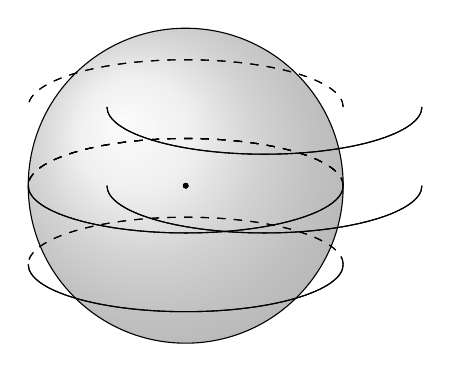
\begin{tikzpicture}
  \shade[ball color = gray!40, opacity = 0.4] (0,0) circle (2cm);
  \draw (0,0) circle (2cm);
  \foreach \i in {1,...,4} {
    \pgfmathtruncatemacro{\y}{2 * \i / 5};
    \pgfmathtruncatemacro{\r}{sqrt(2 - \y*\y)};
    \draw (-\r,\y) arc (180:360:2 and 0.6);
    \draw[dashed] (2,\y) arc (0:180:2 and 0.6);
    \draw (-2,-\y) arc (180:360:2 and 0.6);
    \draw[dashed] (2,-\y) arc (0:180:2 and 0.6);
    \fill[fill=black] (0,0) circle (1pt);
  }
\end{tikzpicture}
\fi


\begin{frame}{Solovay--Kitaev theorem}
\begin{theorem}
Assume $\{U_1,\dotsc,U_k\}$ generates a dense subset of $\mathsf{SU}(2)$.
Then, any $U\in\mathsf{SU}(2)$ can be approxmiated with error $\epsilon$ by $\emm{[\log (1/\epsilon)]^c}$ multiplications of $\{U_1,\dotsc,U_k\}$
for some constant $c$.
\end{theorem}
\end{frame}

\begin{frame}{Assignments}
\begin{enumerate}
\setlength{\itemsep}{2em}
\item 
Show a quantum circuit for controlled-$\begin{bmatrix} 1 & 0\\ 0 & e^{i\theta}\end{bmatrix}$ gate with \emm{two} controlled qubits
using the $\mathsf{CNOT}$ gates and arbitrary single-qubit gates.

\item {[Advanced]}
Show a quantum circuit for controlled-$\begin{bmatrix} 1 & 0\\ 0 & -1\end{bmatrix}$ gate with \emm{two} controlled qubits
using \emm{six} $\mathsf{CNOT}$ gates and \emm{seven} $T$ and $T^\dagger$ gates.
\end{enumerate}
\end{frame}


\end{document}
